%% ============================================================
%% Chapter 2 — Classical Exact Algorithms for the Capacitated
%%             Vehicle Routing Problem
%% Source: Toth & Vigo (eds.), Vehicle Routing: Problems,
%%         Methods, and Applications, 2nd ed., SIAM 2014.
%%         Chapter by Frederic Semet, Paolo Toth, Daniele Vigo.
%% ============================================================
\documentclass[aspectratio=169,10pt]{beamer}

\usetheme{Madrid}
\usecolortheme{seahorse}
\setbeamertemplate{footline}[frame number]
\setbeamertemplate{navigation symbols}{}

%% --- Packages ---
\usepackage[utf8]{inputenc}
\usepackage[T1]{fontenc}
\usepackage{amsmath,amssymb,amsthm}
\usepackage{mathtools}
\usepackage{graphicx}
\usepackage{booktabs}
\usepackage{array}
\usepackage{multirow}
\usepackage{xcolor}
\usepackage{listings}
\usepackage{algorithm}
\usepackage{algpseudocode}
\usepackage{tikz}
\usetikzlibrary{arrows.meta,positioning,shapes.geometric}
\usepackage{hyperref}
\usepackage[expansion=false]{microtype}

\graphicspath{{figures/}}

%% --- Listings style ---
\lstset{
  language=Python,
  basicstyle=\ttfamily\scriptsize,
  numbers=left,
  numberstyle=\tiny\color{gray},
  frame=single,
  backgroundcolor=\color{gray!7},
  commentstyle=\color{green!50!black}\itshape,
  keywordstyle=\color{blue!80!black}\bfseries,
  stringstyle=\color{red!70!black},
  breaklines=true,
  tabsize=4,
  showstringspaces=false,
}

%% --- Math shortcuts ---
\newcommand{\R}{\mathbb{R}}
\newcommand{\Z}{\mathbb{Z}}
\DeclareMathOperator{\argmin}{argmin}
\newcommand{\ceil}[1]{\left\lceil #1 \right\rceil}
\newcommand{\floor}[1]{\left\lfloor #1 \right\rfloor}

%% --- Title ---
\title[Ch.2: Classical Exact CVRP]{%
  \textbf{Chapter 2: Classical Exact Algorithms\\
  for the Capacitated Vehicle Routing Problem}}
\subtitle{Vehicle Routing: Problems, Methods, and Applications\\
          Toth \& Vigo (eds.), 2nd Edition, SIAM 2014}
\author{Fr\'ed\'eric Semet \and Paolo Toth \and Daniele Vigo}
\date{Slides prepared for self-study}

%% ============================================================
\begin{document}
%% ============================================================

\begin{frame}
  \titlepage
\end{frame}

%% ─────────────────────────────────────────────────────────────
\begin{frame}[allowframebreaks]{Chapter Outline}
%% ─────────────────────────────────────────────────────────────
  This chapter surveys the most important exact methods developed
  for the Capacitated Vehicle Routing Problem (CVRP), tracing progress
  from the first Branch-and-Bound algorithms in the late 1960s through
  the state-of-the-art Branch-and-Cut procedures of the 2000s.

  \bigskip
  \tableofcontents
\end{frame}

\AtBeginSection[]{
  \begin{frame}[allowframebreaks]{Section Outline}
    \tableofcontents[currentsection]
  \end{frame}
}

\section{Introduction: Why Exact Methods Matter}
\section{Branch-and-Bound Algorithms}
\section{Early Set Partitioning Algorithms}
\section{Branch-and-Cut Algorithms}
\section{Families of Cuts}
\section{Separation Procedures}
\section{Comparison of B\&C Methods}
\section{Conclusions and Future Directions}
\section{Bibliography}

%% ============================================================
\section{Introduction: Why Exact Methods Matter}
%% ============================================================

\begin{frame}[allowframebreaks]{The Capacitated Vehicle Routing Problem}
  \begin{block}{Problem Definition (CVRP)}
    Given a depot (vertex 0) and a set $V' = \{1,\ldots,n\}$ of customers
    embedded in a graph $G=(V,A)$ with $V=\{0\}\cup V'$, the CVRP asks for
    a minimum-cost set of routes, each starting and ending at the depot, such
    that every customer is visited exactly once and the total demand on each
    route does not exceed the vehicle capacity $Q$.
  \end{block}

  \bigskip
  Each customer $i \in V'$ has a non-negative demand $d_i$.
  A fleet of $m$ identical vehicles, each of capacity $Q$, is available at
  the depot. The cost of travelling from vertex $i$ to vertex $j$ is $c_{ij}$;
  for most benchmark instances $c_{ij}$ is the Euclidean distance between
  customers placed in the plane.

  \framebreak

  \begin{columns}
    \begin{column}{0.52\textwidth}
      
\includegraphics[width=\textwidth]{cvrp_example}
    \end{column}
    \begin{column}{0.46\textwidth}
      \textbf{Example:} Six customers with demands shown. Vehicle capacity $Q=12$.
      \begin{itemize}
        \item Route 1 (blue): depot $\to c_1 \to c_2 \to c_3 \to$ depot.
              Total demand $3+4+3=10 \leq 12$. \checkmark
        \item Route 2 (orange): depot $\to c_4 \to c_5 \to c_6 \to$ depot.
              Total demand $5+4+3=12 \leq 12$. \checkmark
      \end{itemize}
      The objective is to minimise the total travel cost (sum of arc costs)
      over all routes.
    \end{column}
  \end{columns}

  \framebreak

  \begin{block}{CVRP as a Mixed-Integer Program}
    Introduce binary variable $x_{ij} \in \{0,1\}$ equal to 1 if a vehicle
    travels directly from vertex $i$ to vertex $j$, and 0 otherwise.
    Let $x(\delta(S)) = \sum_{(i,j)\in\delta(S)} x_{ij}$ denote the number
    of arcs leaving subset $S\subseteq V$.

    \begin{align}
      \min \quad   & \sum_{(i,j)\in A} c_{ij}\, x_{ij} \tag{P}\\
      \text{s.t.}\ & x(\delta(\{i\})) = 2, \quad \forall\, i \in V' \label{eq:deg}\\
                   & x(\delta(S)) \geq 2\ceil{d(S)/Q},\quad \forall\, S\subseteq V',\;S\neq\emptyset \label{eq:cap}\\
                   & x_{ij} \in \{0,1\},\quad \forall\,(i,j)\in A \label{eq:bin}
    \end{align}
  \end{block}

  Constraint \eqref{eq:deg} ensures that every customer is visited
  exactly once (degree-2 condition). Constraint \eqref{eq:cap} is the
  \emph{rounded capacity inequality} (RCI): it guarantees that at least
  $\lceil d(S)/Q \rceil$ vehicles service the customer set $S$, so at least
  $2\lceil d(S)/Q\rceil$ arcs must cross the boundary $\delta(S)$.
  The RCI simultaneously eliminates sub-tours and enforces capacity feasibility.

  \framebreak

  \begin{alertblock}{Key Insight: Why Exact Methods Are Difficult}
    The CVRP is NP-hard in the strong sense: no polynomial-time algorithm
    is known, and decades of research suggest none exists. However, exact
    algorithms are \emph{indispensable} because:
    \begin{enumerate}
      \item They provide \textbf{certified optimal solutions} that validate
            the quality of heuristics.
      \item They supply \textbf{tight lower bounds} used to assess the
            optimality gap of practical solutions.
      \item Modern B\&C can now solve instances with up to 135--200 customers
            to proven optimality, covering many real-world scenarios.
    \end{enumerate}
  \end{alertblock}

  \bigskip
  The chapter is organised in three sections: Section 2.2 covers
  Branch-and-Bound; Section 2.3 covers Set Partitioning formulations solved
  by column generation; Section 2.4 covers Branch-and-Cut, the dominant
  approach today.
\end{frame}

%% ============================================================
\section{Branch-and-Bound Algorithms}
%% ============================================================

\begin{frame}[allowframebreaks]{Branch-and-Bound: Core Idea}
  Branch-and-Bound (B\&B) solves a combinatorial optimisation problem by
  \emph{implicitly} enumerating all feasible solutions.
  The key insight is that large portions of the search space can be
  \textbf{pruned}---discarded without explicit examination---whenever a
  \emph{lower bound} on the cost of any solution reachable from the current
  node is at least as large as the cost of the best solution found so far
  (the \emph{upper bound}).

  \bigskip
  The algorithm maintains a tree of \emph{subproblems}. Each node in the
  tree corresponds to a subproblem obtained by fixing some variables (e.g.,
  setting $x_{ij}=1$ or $x_{ij}=0$). The root node is the full, unfixed
  problem. Leaf nodes are either infeasible, pruned, or correspond to a
  complete integer solution.

  \framebreak

  \begin{columns}
    \begin{column}{0.54\textwidth}
      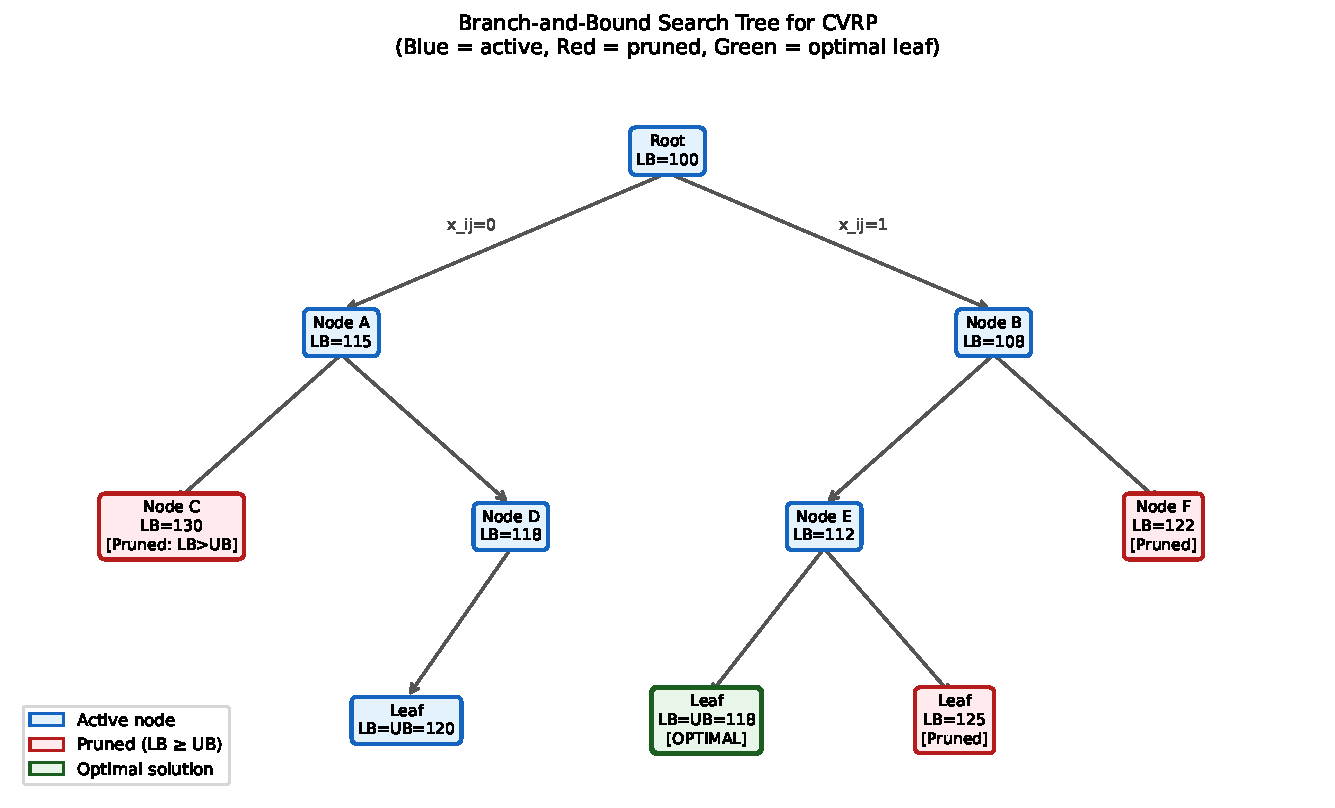
\includegraphics[width=\textwidth]{bnb_tree}
    \end{column}
    \begin{column}{0.44\textwidth}
      \textbf{Three pruning criteria:}
      \begin{enumerate}
        \item \textbf{Infeasibility}: the node's subproblem has no feasible
              solution.
        \item \textbf{Bound}: the node's lower bound LB $\geq$ current upper
              bound UB. No better solution can lie in this subtree.
        \item \textbf{Optimality}: the LP solution is already integer --- it
              is a feasible CVRP solution. Update UB if it improves the
              incumbent.
      \end{enumerate}
      In the figure, red nodes are pruned by criterion 2 (LB $\geq$ UB=120),
      and the green leaf with LB=UB=118 is the \textbf{optimal solution}.
    \end{column}
  \end{columns}

  \framebreak

  \begin{block}{Generic B\&B Algorithm for CVRP}
    \begin{algorithmic}[1]
      \State Initialise: $UB \leftarrow$ cost of a heuristic solution;
             open-list $\mathcal{L} \leftarrow \{\text{root node}\}$.
      \While{$\mathcal{L} \neq \emptyset$}
        \State Select and remove a node $N$ from $\mathcal{L}$.
        \State Compute lower bound $LB(N)$ for node $N$.
        \If{$LB(N) \geq UB$} \textbf{prune} $N$; \textbf{continue}.
        \EndIf
        \If{LP solution at $N$ is integer and feasible}
          \State Update $UB \leftarrow LB(N)$; record solution; \textbf{continue}.
        \EndIf
        \State \textbf{Branch}: select a fractional variable $x_{ij}$; create
               two children by adding constraint $x_{ij}=0$ or $x_{ij}=1$;
               add both to $\mathcal{L}$.
      \EndWhile
      \State \Return best solution found with cost $UB$.
    \end{algorithmic}
  \end{block}

  \framebreak

  \begin{alertblock}{Key Insight: Lower Bounds Drive B\&B Efficiency}
    The quality of the lower bound is the single most important factor
    in B\&B performance. A tight LB prunes more nodes and leads to faster
    convergence. For the CVRP, effective lower bounds come from LP relaxations
    (solved once per node) and problem-specific relaxations such as the
    Assignment Problem (AP) and the \emph{q}-routes relaxation.
  \end{alertblock}
\end{frame}

\begin{frame}[allowframebreaks]{2.2.1 Assignment and Matching Relaxations}
  The assignment and matching-based bounds, pioneered by Christofides and
  Eilon (1969) and refined by Toth and Vigo, provide fast lower bounds
  exploiting the structure of the CVRP.

  \bigskip
  \textbf{Assignment Problem (AP) relaxation.} The AP is obtained from the
  CVRP by dropping the capacity constraints and the sub-tour elimination
  constraints: we merely require each vertex to have in-degree 1 and
  out-degree 1. The AP is solvable in $O(n^3)$ time (Hungarian algorithm)
  and its optimal value is a lower bound for the CVRP. However, the AP
  solution often contains sub-tours, as illustrated below.

  \bigskip
  \begin{columns}
    \begin{column}{0.55\textwidth}
      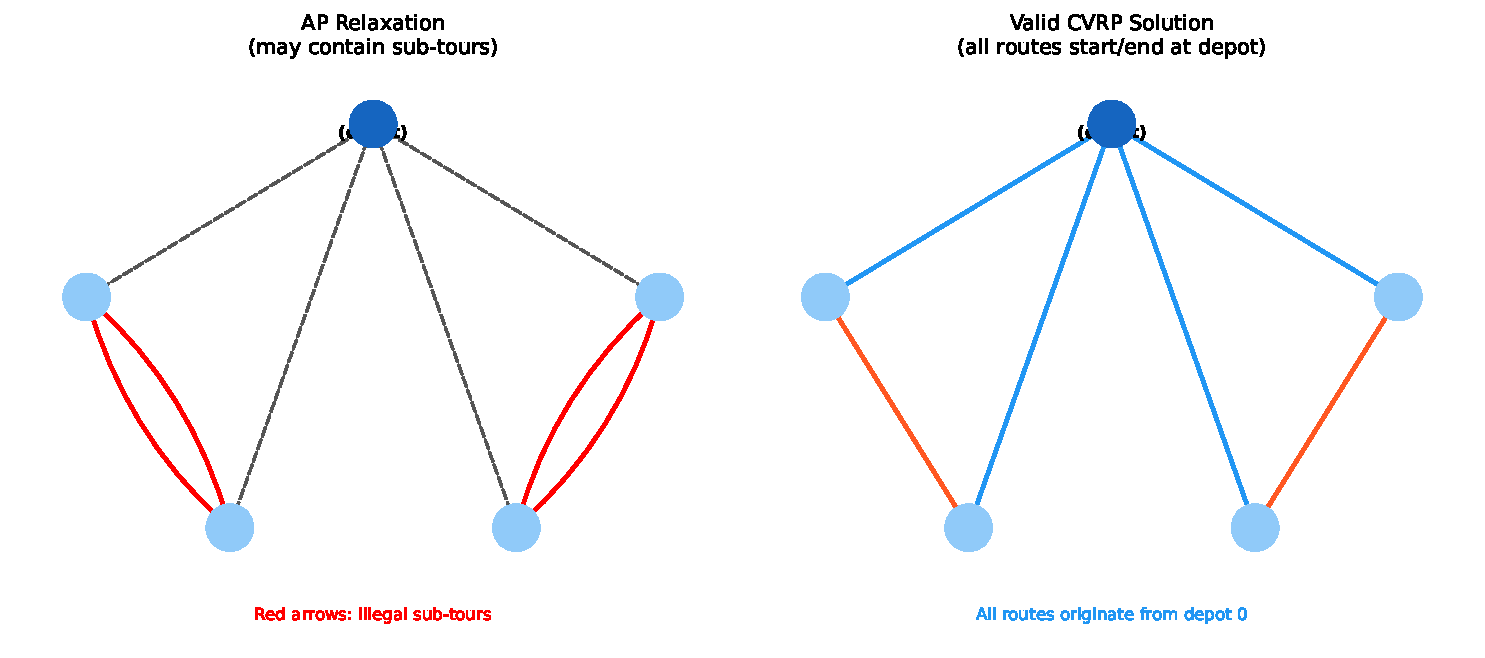
\includegraphics[width=\textwidth]{ap_relaxation}
    \end{column}
    \begin{column}{0.43\textwidth}
      \textbf{Left}: AP solution for 5 customers. Two sub-tours
      $\{1\to 2\to 1\}$ and $\{3\to 4\to 3\}$ are formed (red arrows)
      which are \emph{infeasible} for CVRP.

      \textbf{Right}: A valid CVRP solution with all routes starting/ending
      at the depot.

      The AP lower bound is used as the \emph{root bound} $z_{AP}$ in the
      B\&B tree; any CVRP solution has cost $\geq z_{AP}$.
    \end{column}
  \end{columns}

  \framebreak

  \textbf{The \emph{q}-routes relaxation.} Introduced by Christofides, Mingozzi,
  and Toth (1981), this relaxation generates a stronger lower bound by
  replacing each CVRP route with a shortest Hamiltonian path from the depot
  to vertex $k$ using at most $q$ edges, where $k$ varies over all customers.
  It is formulated as a shortest-path problem on an acyclic graph and solved
  in pseudo-polynomial time. When $q=2$ (allowing 1 intermediate customer),
  the bound is already substantially tighter than the AP bound.

  \bigskip
  \textbf{In the B\&B framework}, the lower bound at each node is computed
  by:
  \begin{enumerate}
    \item Solving the AP relaxation of the \emph{reduced} subproblem
          (with fixed arcs incorporated), yielding bound $z_{AP}$.
    \item Optionally adding the $q$-routes component to tighten $z_{AP}$.
    \item Using the combined bound as the node's LB.
  \end{enumerate}

  The overall AP additive approach (Christofides and Eilon, 1969) solved
  problems up to $n=50$ customers. The refinements of Fisher (1994) and
  Toth and Vigo (2002) extended the reach to $n=100$.

  \framebreak

  \begin{exampleblock}{Worked Example: AP Relaxation for 4 Customers}
    Consider a CVRP with depot 0 and customers $\{1,2,3,4\}$ and the
    following cost matrix (symmetric, $c_{ij}=c_{ji}$):
    \[
      C = \begin{pmatrix}
            - & 4 & 8 & 6 & 5 \\
            4 & - & 3 & 7 & 9 \\
            8 & 3 & - & 5 & 4 \\
            6 & 7 & 5 & - & 2 \\
            5 & 9 & 4 & 2 & -
          \end{pmatrix}, \quad Q=6, \quad d_1=3,\;d_2=3,\;d_3=4,\;d_4=4.
    \]
    The AP relaxation assigns each vertex a unique successor. One AP
    optimal assignment might yield:
    $0\to 1$, $1\to 2$, $2\to 0$, $3\to 4$, $4\to 3$ with cost
    $4+3+8+2+2=19$. This contains the sub-tour $\{3\to 4\to 3\}$.
    Hence $z_{AP}=19$ is a \emph{lower bound} for the CVRP.

    A valid CVRP solution: route $A$: $0\to 1\to 2\to 0$ (cost $4+3+8=15$,
    demand $3+3=6\leq Q$); route $B$: $0\to 3\to 4\to 0$ (cost $6+2+5=13$,
    demand $4+4=8>Q$). Infeasible! Try: route $B'$: $0\to 3\to 0$ (cost
    $6+6=12$, demand $4$); route $C$: $0\to 4\to 0$ (cost $5+5=10$, demand
    $4$). Total cost $=15+12+10=37$. The AP bound $z_{AP}=19$ is far from
    this, showing the bound's weakness. Adding capacity penalties tightens it.
  \end{exampleblock}
\end{frame}

\begin{frame}[allowframebreaks]{2.2.2 Bounds Based on Spanning and Additive Approaches}
  Beyond the AP relaxation, several bounding strategies improve the lower
  bound by incorporating capacity constraints more tightly. Two important
  approaches are the \emph{spanning} bounds and the \emph{additive} approach.

  \bigskip
  \textbf{Spanning tree bound.} The 1-tree relaxation (used for the TSP by
  Held and Karp, 1971) can be adapted for the CVRP. One removes the depot,
  computes a minimum spanning tree of the customer graph, and then attaches
  the two cheapest depot edges to each customer at the ``ends'' of the tree.
  This gives a lower bound because every CVRP tour, when the depot is
  removed, induces a Hamiltonian path (a special spanning tree).

  \bigskip
  \textbf{Lagrangian relaxation.} A more powerful approach dualises the
  degree constraints or capacity constraints by adding them to the objective
  with Lagrange multipliers $\lambda_i$. For multiplier vector $\lambda$,
  the Lagrangian relaxation $LR(\lambda)$ provides a lower bound:
  \[
    LB(\lambda) = \min_{x \geq 0,\;x\text{ feasible for relaxed problem}}
                  \Bigl[\sum_{(i,j)} c_{ij} x_{ij}
                        + \sum_i \lambda_i\bigl(x(\delta(\{i\}))-2\bigr)\Bigr].
  \]
  The \emph{Lagrangian dual} $\max_\lambda LB(\lambda)$ is solved by
  subgradient optimisation. At each step the multipliers are updated as
  $\lambda_i \leftarrow \lambda_i + t_k(x(\delta(\{i\}))-2)$, where $t_k$
  is a step size satisfying $\sum_k t_k = \infty$ and $\sum_k t_k^2 < \infty$.

  \framebreak

  \textbf{Additive approach.} The additive bounding procedure, described
  by Toth and Vigo (2002), combines several relaxations additively. Let
  $z_1$ be the AP lower bound. One then computes corrections:
  \[
    z_{\text{add}} = z_1 + z_2 + \cdots + z_k,
  \]
  where each $z_\ell$ is a ``correction term'' obtained by solving a
  sub-problem that accounts for features not captured in $z_{\ell-1}$.
  For example, $z_2$ may account for the minimum cost of ensuring that
  at least two arcs leave the depot (i.e., at least one vehicle exists).
  This additive scheme gives bounds significantly tighter than the AP
  bound alone without the computational cost of solving the full LP.

  \bigskip
  \begin{alertblock}{Key Insight: Additive vs.\ LP Bounds}
    The additive AP-based bounds run in $O(n^3)$ time per node, whereas
    LP relaxations (using interior point or simplex) can be much slower.
    Early B\&B algorithms (1969--2002) therefore preferred AP-based
    bounds. Modern B\&C algorithms use LP bounds enhanced by cutting planes,
    which are far tighter and justify the higher computational cost.
  \end{alertblock}
\end{frame}

\begin{frame}[allowframebreaks]{2.2.3 Branch-and-Bound Branching Strategies}
  The choice of which variable to branch on, and the order in which nodes
  are explored, profoundly affect B\&B performance. For the CVRP, several
  branching rules have been proposed.

  \bigskip
  \textbf{Branching on arc variables.} The most natural rule selects a
  fractional arc variable $x_{ij}$ and creates two child nodes: one with
  $x_{ij}=1$ (the arc is used) and one with $x_{ij}=0$ (the arc is
  forbidden). The fractional variable closest to $\frac{1}{2}$ is often
  chosen to maximise the difference between the two children.

  \bigskip
  \textbf{Branching on the number of vehicles.} Because the number of
  routes $m$ is a key parameter, branching on $m$ is effective when the
  LP relaxation yields a non-integer $m$. The two children fix $m \leq
  \lfloor m^* \rfloor$ and $m \geq \lceil m^* \rceil$ respectively.

  \bigskip
  \textbf{Node selection strategies:}
  \begin{itemize}
    \item \textbf{Best-first}: always expand the node with the smallest LB.
          Minimises the number of nodes explored but may use much memory.
    \item \textbf{Depth-first}: expand the most recently created node (stack).
          Finds integer solutions quickly, uses less memory, but may explore
          poor subtrees.
    \item \textbf{Best-first with depth-first dives}: a hybrid that dives
          depth-first from the best node, then backtracks.
  \end{itemize}

  \framebreak

  \textbf{Dominance and reduction rules.} Several CVRP-specific reductions
  can be applied at each node to simplify the subproblem:

  \begin{enumerate}
    \item \textbf{Arc elimination}: if $c_{ij}$ is too large (i.e., the
          reduced cost of $x_{ij}$ exceeds $UB - LB$), set $x_{ij}=0$.
    \item \textbf{Forced arcs}: if a vertex $i$ has all but one incident arc
          eliminated, force the remaining arc.
    \item \textbf{Capacity pruning}: if fixing $x_{ij}=1$ would make any
          route demand exceed $Q$, set $x_{ij}=0$.
  \end{enumerate}

  These reductions shrink the problem at each node and significantly reduce
  the branching factor.

  \bigskip
  \begin{block}{Historical Context}
    The B\&B framework for CVRP was first proposed by Christofides and Eilon
    (1969) and solved instances up to $n=50$. Subsequent improvements by
    Laporte, Mercure, and Nobert (1986) used a strengthened bounding procedure
    and reached $n=100$. Toth and Vigo (2002) further refined the approach.
    All these algorithms were eventually superseded by B\&C methods, which
    exploit cutting planes for much tighter bounds.
  \end{block}
\end{frame}

%% ============================================================
\section{Early Set Partitioning Algorithms}
%% ============================================================

\begin{frame}[allowframebreaks]{2.3 Set Partitioning Formulation}
  An alternative to the arc-variable formulation is the
  \emph{Set Partitioning} (SP) formulation, which works with
  \emph{route variables} rather than arc variables. This formulation was
  introduced by Balinski and Quandt (1964) for the TSP and adapted to the
  CVRP by Bramel and Simchi-Levi (1997) and others.

  \bigskip
  \textbf{Idea.} Enumerate (or generate implicitly) all feasible routes
  $r \in \mathcal{R}$. Each route $r$ has a cost $c_r$ and a binary parameter
  $a_{ir} \in \{0,1\}$ equal to 1 if customer $i$ is on route $r$. Choose a
  minimum-cost subset of routes that covers every customer exactly once.

  \begin{block}{Set Partitioning (SP) Model}
    \begin{align}
      \min \quad   & \sum_{r \in \mathcal{R}} c_r\, y_r \tag{SP} \\
      \text{s.t.}\ & \sum_{r \in \mathcal{R}} a_{ir}\, y_r = 1,
                     \quad \forall\, i \in V' \label{eq:sp-cover}\\
                   & y_r \in \{0,1\}, \quad \forall\, r \in \mathcal{R}
                     \label{eq:sp-bin}
    \end{align}
  \end{block}

  Here $y_r=1$ means route $r$ is selected. Constraint \eqref{eq:sp-cover}
  ensures each customer is served by exactly one route. Capacity constraints
  are embedded in $\mathcal{R}$ (only feasible routes are included). The
  formulation is exact but has an exponential number of columns $|\mathcal{R}|$.

  \framebreak

  \begin{columns}
    \begin{column}{0.52\textwidth}
      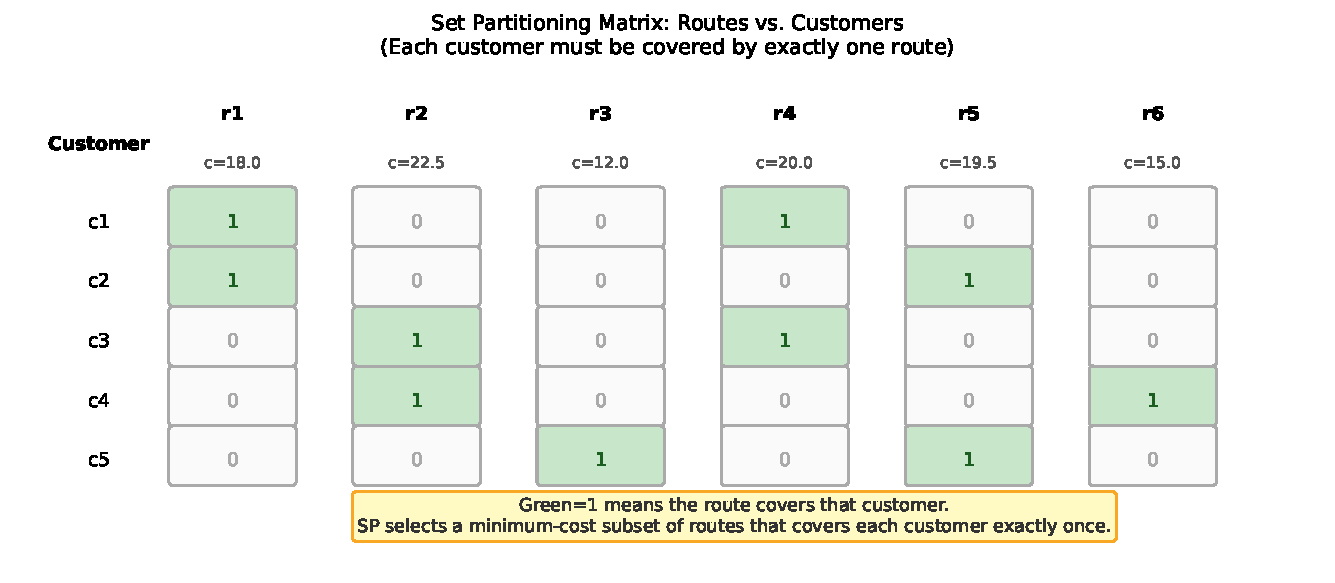
\includegraphics[width=\textwidth]{set_partitioning}
    \end{column}
    \begin{column}{0.46\textwidth}
      \textbf{Set Partitioning Matrix} for 5 customers and 6 candidate routes.
      Each column is a route; each row is a customer. A cell is 1 (green) if
      the route visits that customer.

      The SP problem selects a minimum-cost subset of columns such that each
      row has exactly one selected entry. In this example, selecting routes
      $r_1$, $r_2$, $r_3$ (total cost $18+22.5+12=52.5$) covers all 5
      customers exactly once.
    \end{column}
  \end{columns}

  \framebreak

  \begin{exampleblock}{Worked Example: SP Feasibility Check}
    Suppose we have 4 customers with demands $d_1=3,d_2=4,d_3=3,d_4=5$ and
    capacity $Q=8$. The candidate routes and their coverage are:
    \begin{center}
    \begin{tabular}{llcc}
      \toprule
      Route & Customers & Total Demand & Cost \\
      \midrule
      $r_1$ & $\{1,2\}$   & 7 $\leq$ 8 & 12 \\
      $r_2$ & $\{3,4\}$   & 8 $\leq$ 8 & 15 \\
      $r_3$ & $\{1,3\}$   & 6 $\leq$ 8 & 11 \\
      $r_4$ & $\{2,4\}$   & 9 $>$ 8    & --- (infeasible) \\
      $r_5$ & $\{1,2,3\}$ & 10 $>$ 8   & --- (infeasible) \\
      $r_6$ & $\{4\}$     & 5 $\leq$ 8 & 9  \\
      \bottomrule
    \end{tabular}
    \end{center}
    Feasible SP solutions: $\{r_1, r_2\}$ (cost 27), $\{r_3, r_4\}$
    (infeasible — $r_4$ dropped), $\{r_3, r_6, r_2^*\}$ where $r_2^*$
    covers $\{3,4\}$ minus already-served $\{3\}$. The optimal is
    $\{r_1, r_2\}$ with cost 27.
  \end{exampleblock}
\end{frame}

\begin{frame}[allowframebreaks]{Column Generation for SP LP Relaxation}
  Since $|\mathcal{R}|$ is exponential, the LP relaxation of SP cannot be
  solved by simply loading all columns. Instead, the \emph{column generation}
  technique is used: start with a small \emph{restricted} set of routes
  (the \emph{Restricted Master Problem}, RMP), solve the LP, then iteratively
  add routes (columns) that improve the objective.

  \bigskip
  \textbf{How column generation works.} At each iteration:
  \begin{enumerate}
    \item Solve the LP relaxation of the RMP. Let $\pi_i$ be the optimal
          dual variable (shadow price) for customer $i$'s covering constraint.
    \item Compute the \emph{reduced cost} of each route $r \notin$ RMP:
          \[
            \bar{c}_r = c_r - \sum_{i \in V'} \pi_i\, a_{ir}.
          \]
          A route improves the LP objective if and only if $\bar{c}_r < 0$.
    \item Find the route with minimum reduced cost (the \emph{pricing
          subproblem}). If $\bar{c}_r \geq 0$ for all routes, the current
          LP solution is optimal for the full SP LP.
    \item Otherwise, add the most negative-reduced-cost route to the RMP
          and repeat.
  \end{enumerate}

  \framebreak

  \begin{columns}
    \begin{column}{0.56\textwidth}
      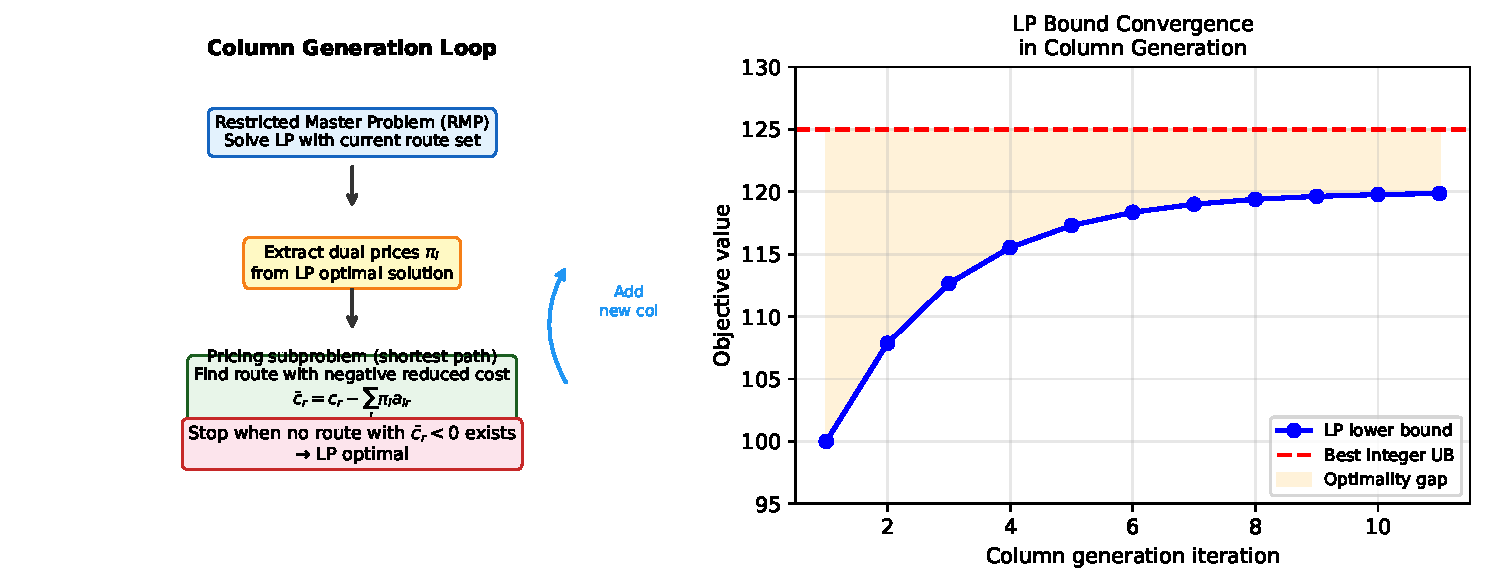
\includegraphics[width=\textwidth]{column_generation}
    \end{column}
    \begin{column}{0.42\textwidth}
      \textbf{Left}: the column generation loop. The dual prices $\pi_i$
      from the RMP guide the pricing subproblem: find the cheapest route
      considering these shadow prices.

      \textbf{Right}: convergence of the LP lower bound. After 10--15
      column generation iterations the bound stabilises near the optimum.
      The orange gap between the LP bound and the integer UB is the
      \emph{optimality gap}.
    \end{column}
  \end{columns}

  \framebreak

  \textbf{The pricing subproblem for CVRP.} Finding the route with minimum
  reduced cost is equivalent to finding a minimum-cost elementary path
  (visiting each customer at most once) from the depot back to the depot,
  with total demand $\leq Q$. This is a \emph{resource-constrained shortest
  path problem} (ESPPRC), which is itself NP-hard in general. In practice:
  \begin{itemize}
    \item Dynamic programming on a state space $(i, S, d)$, where $i$ is the
          current customer, $S$ is the set of visited customers, and $d$ is
          the accumulated demand.
    \item \emph{Non-elementary relaxation}: allow repeated customers
          (easier to solve), giving routes that may visit a customer multiple
          times. Used in early implementations (Agarwal et al., 1989).
    \item \emph{ng-routes} (Baldacci, Mingozzi, Roberti, 2011): a compromise
          allowing bounded non-elementarity, widely used in modern B\&C.
  \end{itemize}

  \framebreak

  \begin{block}{Historical SP Algorithms for CVRP}
    \begin{itemize}
      \item \textbf{Agarwal, Mathur, and Salkin (1989)}: first practical SP
            algorithm for CVRP. Used column generation without branch-and-bound.
            Solved instances up to $n=45$.
      \item \textbf{Desrochers, Desrosiers, and Solomon (1992)}: rigorous
            column generation with ESPPRC pricing. Extended to VRPTW.
      \item \textbf{Fisher and Jaikumar (1981)}: generalised assignment
            heuristic that inspired later exact SP algorithms.
    \end{itemize}
  \end{block}

  \begin{alertblock}{Key Insight: Column Generation Provides LP Bound}
    The LP relaxation of SP solved by column generation gives a lower bound
    at least as tight as the LP relaxation of the arc-variable formulation,
    and often much tighter. This makes SP-based B\&C methods highly
    competitive.
  \end{alertblock}
\end{frame}

%% ============================================================
\section{Branch-and-Cut Algorithms}
%% ============================================================

\begin{frame}[allowframebreaks]{2.4 Branch-and-Cut: The Dominant Approach}
  Branch-and-Cut (B\&C) is today the most powerful exact approach for
  combinatorial optimisation problems with a rich polyhedral structure,
  including the CVRP. The method was developed for the TSP by Padberg and
  Rinaldi (1991) and extended to the CVRP by Padberg and Rinaldi (1991),
  Laporte et al.\ (1986), and most influentially by Augerat et al.\ (1995)
  and Lysgaard et al.\ (2004).

  \bigskip
  \textbf{Core idea.} B\&C combines the B\&B tree search with an LP relaxation
  that is \emph{progressively tightened} at each node by adding cutting planes
  (\emph{valid inequalities}). A valid inequality is a linear constraint
  satisfied by \emph{all} integer feasible CVRP solutions but violated by the
  current fractional LP solution. Adding it ``cuts off'' the fractional point,
  tightening the LP relaxation and raising the lower bound.

  \framebreak

  \begin{columns}
    \begin{column}{0.46\textwidth}
      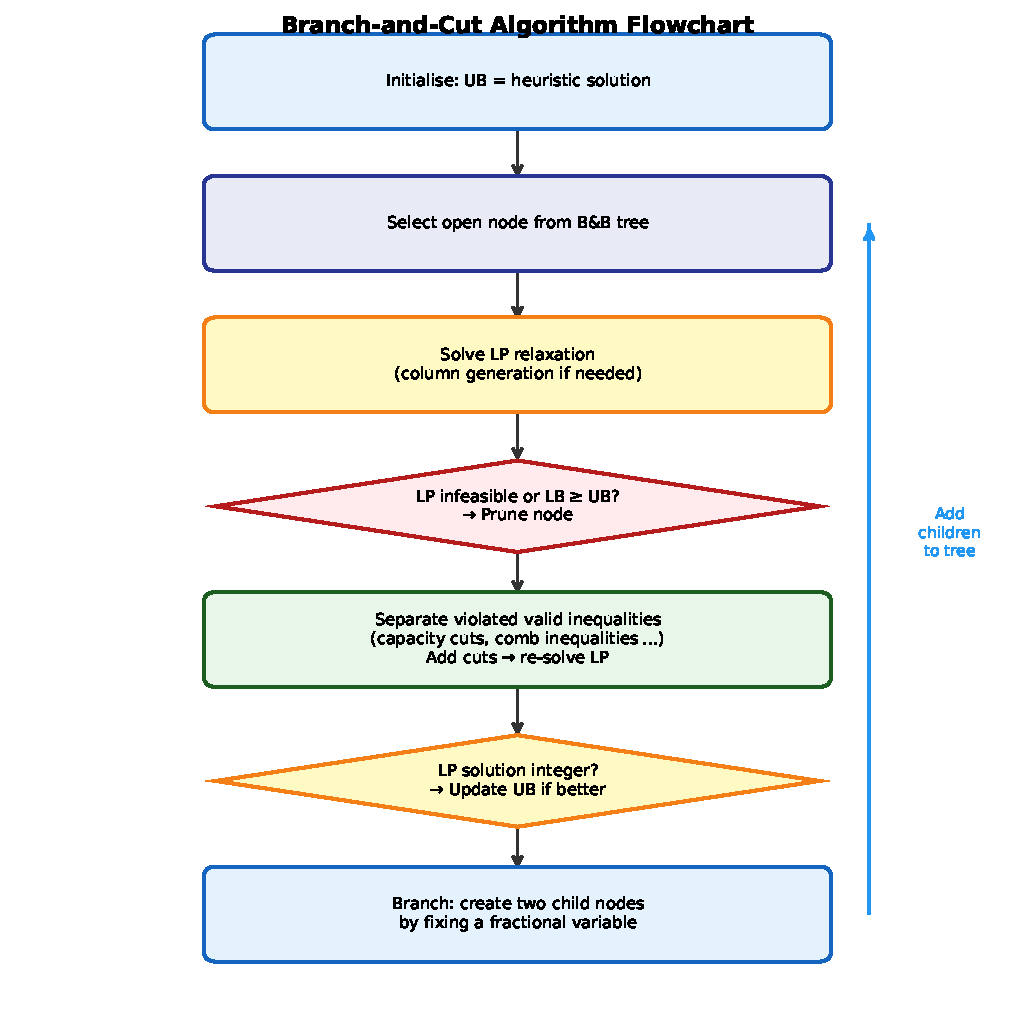
\includegraphics[width=\textwidth]{branch_cut_flow}
    \end{column}
    \begin{column}{0.52\textwidth}
      \textbf{B\&C Algorithm Overview:}
      \begin{enumerate}
        \item \textbf{Initialise} with a heuristic upper bound $UB$.
        \item \textbf{Select} an open node from the B\&B tree.
        \item \textbf{Solve LP relaxation} at the node (reusing cuts from
              the parent node).
        \item \textbf{Prune} if LP infeasible or $LB \geq UB$.
        \item \textbf{Separate}: find violated valid inequalities; add them
              to the LP and re-solve. Repeat until no violated inequality is
              found or a limit is reached.
        \item If LP solution is \textbf{integer}: update $UB$ if better.
        \item Otherwise, \textbf{branch} on a fractional variable.
        \item \textbf{Add children} to the tree; repeat.
      \end{enumerate}
    \end{column}
  \end{columns}

  \framebreak

  \begin{alertblock}{Why B\&C Dominates B\&B for CVRP}
    Pure B\&B relies on LP relaxations that may be very weak (large gap between
    LP bound and integer optimum). B\&C tightens the LP relaxation by adding
    cutting planes, so:
    \begin{itemize}
      \item Fewer B\&B nodes need to be explored.
      \item The LP bound at the root node may already be very close to the
            optimum, sometimes proving optimality without branching.
      \item State-of-the-art B\&C (Lysgaard et al., 2004) solves instances
            up to 135 customers routinely.
    \end{itemize}
  \end{alertblock}
\end{frame}

%% ============================================================
%% Running Example: B&C Trace
%% ============================================================

\begin{frame}[allowframebreaks]{Running Example: Branch-and-Cut Step by Step}

  We trace B\&C on a \emph{tiny} instance to make every step concrete:
  how a fractional LP solution is identified, which RCI is violated,
  how the cut is derived algebraically, and how the lower bound climbs
  until it meets the upper bound.

  \begin{columns}
    \begin{column}{0.46\textwidth}
      \begin{block}{Instance — 3 customers, $Q=7$}
        \begin{tabular}{@{}ll@{}}
          Demands: & $d_1=3,\;d_2=4,\;d_3=4$ \\[2pt]
          Depot arcs: & $c_{01}=10,\;c_{02}=8,\;c_{03}=12$ \\[2pt]
          Cust.\ arcs: & $c_{12}=5,\;c_{13}=9,\;c_{23}=7$
        \end{tabular}

        \medskip
        Total demand $=11$, so $r(V')=\lceil 11/7\rceil=2$ vehicles needed.

        \smallskip
        \textbf{Heuristic UB.} Route $0\!\to\!1\!\to\!2\!\to\!0$
        (cost $10+5+8=23$, demand $7\leq Q$) $+$ route $0\!\to\!3\!\to\!0$
        (cost $24$, demand $4$): $\boldsymbol{UB=47}$.
      \end{block}
    \end{column}
    \begin{column}{0.52\textwidth}
      \begin{center}
      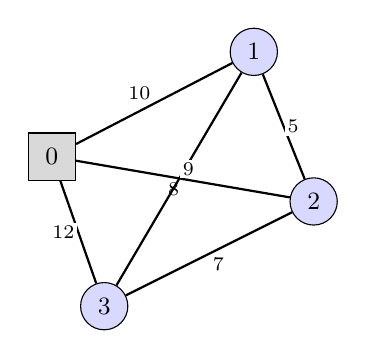
\begin{tikzpicture}[scale=0.95,
          depot/.style={draw,rectangle,fill=gray!30,minimum size=0.6cm,font=\small\bfseries},
          cust/.style={draw,circle,fill=blue!15,minimum size=0.6cm,font=\small\bfseries},
          lbl/.style={font=\scriptsize,fill=white,inner sep=1pt}]
        \node[depot] (0) at (0.5,0)    {$0$};
        \node[cust]  (1) at (3.2,1.4)  {$1$};
        \node[cust]  (2) at (4.0,-0.6) {$2$};
        \node[cust]  (3) at (1.2,-2.0) {$3$};
        \draw[thick] (0)--(1) node[lbl,midway,above left]{10};
        \draw[thick] (0)--(2) node[lbl,midway,below left]{8};
        \draw[thick] (0)--(3) node[lbl,midway,left]{12};
        \draw[thick] (1)--(2) node[lbl,midway,right]{5};
        \draw[thick] (1)--(3) node[lbl,midway,above right]{9};
        \draw[thick] (2)--(3) node[lbl,midway,below right]{7};
      \end{tikzpicture}
      \end{center}
    \end{column}
  \end{columns}

  \framebreak

  %% ---- Step 1: Initial LP ----------------------------------------
  \textbf{Step 1 — LP relaxation (degree constraints only, no RCIs yet).}

  \smallskip
  Variable $x_{ij}\geq 0$ = fraction of time edge $(i,j)$ is used.
  Degree constraints: $x_{01}+x_{12}+x_{13}=2$,\;
  $x_{02}+x_{12}+x_{23}=2$,\; $x_{03}+x_{13}+x_{23}=2$.

  Substituting these into the objective (to eliminate $x_{01},x_{02},x_{03}$):
  \[
    z \;=\; 60 \;-\; 13\,(x_{12}+x_{13}+x_{23}).
  \]
  The LP \emph{maximises} the sum of inter-customer edges.
  Setting $x_{12}=x_{13}=x_{23}=1$ satisfies all three degree constraints with
  $x_{01}=x_{02}=x_{03}=0$, giving:
  \[
    \boxed{z_{LP}^{(0)}=21,\quad LB=21.}
    \qquad\text{Gap }=47-21=26.
  \]

  \begin{columns}
    \begin{column}{0.38\textwidth}
      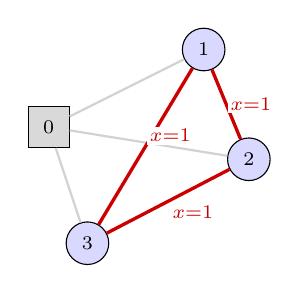
\begin{tikzpicture}[scale=0.82,
          depot/.style={draw,rectangle,fill=gray!30,minimum size=0.52cm,font=\scriptsize\bfseries},
          cust/.style={draw,circle,fill=blue!15,minimum size=0.52cm,font=\scriptsize\bfseries},
          lbl/.style={font=\scriptsize,fill=white,inner sep=1pt}]
        \node[depot] (0) at (0.4,0)    {$0$};
        \node[cust]  (1) at (2.8,1.2)  {$1$};
        \node[cust]  (2) at (3.5,-0.5) {$2$};
        \node[cust]  (3) at (1.0,-1.8) {$3$};
        \draw[gray!35,thick] (0)--(1);
        \draw[gray!35,thick] (0)--(2);
        \draw[gray!35,thick] (0)--(3);
        \draw[red!80!black,very thick] (1)--(2) node[lbl,midway,right]{$x{=}1$};
        \draw[red!80!black,very thick] (1)--(3) node[lbl,midway,above right]{$x{=}1$};
        \draw[red!80!black,very thick] (2)--(3) node[lbl,midway,below right]{$x{=}1$};
      \end{tikzpicture}
    \end{column}
    \begin{column}{0.60\textwidth}
      \textbf{Problem:} The LP solution is the sub-tour $\{1\text{--}2\text{--}3\}$
      with \emph{no depot arcs at all}!
      Although each customer has degree 2 (constraint satisfied), this is
      clearly not a valid CVRP solution.
      We need RCIs to cut off this infeasible point.
    \end{column}
  \end{columns}

  \framebreak

  %% ---- Step 2: First cut -----------------------------------------
  \textbf{Step 2 — Separation: find the most violated RCI.}

  \smallskip
  For each subset $S\subseteq V'$ compute $x(\delta(S))$ and check $x(\delta(S))\geq 2r(S)$.

  Try $S=\{2,3\}$:\; $d(S)=4+4=8$,\; $r(S)=\lceil 8/7\rceil=2$.
  \[
    x\!\left(\delta(\{2,3\})\right)
      = \underbrace{x_{02}+x_{03}}_{\text{depot--}S\text{ boundary}}
      + \underbrace{x_{12}+x_{13}}_{\text{cust.~1--}S\text{ boundary}}
      = 0+0+1+1 = 2 \;<\; 2r(S)=4.
    \quad\textbf{VIOLATED.}
  \]
  \textbf{Add cut} (RCI for $S=\{2,3\}$):
  $\boldsymbol{x_{02}+x_{03}+x_{12}+x_{13}\geq 4}$.

  \medskip
  \textbf{LP after Cut 1.}\;
  Substitute the degree equations for $x_{02}$ and $x_{03}$:
  \[
    (2-x_{12}-x_{23})+(2-x_{13}-x_{23})+x_{12}+x_{13}\;\geq\;4
    \;\;\Longrightarrow\;\;
    4-2x_{23}\geq 4
    \;\;\Longrightarrow\;\;
    x_{23}=0.
  \]
  With $x_{23}=0$, the LP maximises $x_{12}+x_{13}$ giving $x_{12}=x_{13}=1$,
  $x_{01}=0$, $x_{02}=x_{03}=1$.
  \[
    \boxed{z_{LP}^{(1)} = 8+12+5+9 = 34,\quad LB=34.}
    \qquad\text{Gap }=47-34=13.
  \]
  The solution is the Hamiltonian cycle $0\!\to\!2\!\to\!1\!\to\!3\!\to\!0$
  (demand $4+3+4=11>Q$).  One route cannot serve all 3 customers ---
  but the LP does not know this yet.  We need another cut.

  \framebreak

  %% ---- Step 3: Second cut ----------------------------------------
  \textbf{Step 3 — Separation again (re-check all subsets).}

  \smallskip
  Try $S=\{1,2,3\}=V'$:\; $d(S)=11$,\; $r(S)=\lceil 11/7\rceil=2$.
  \[
    x\!\left(\delta(V')\right) = x_{01}+x_{02}+x_{03} = 0+1+1 = 2 \;<\; 2r(S)=4.
    \quad\textbf{VIOLATED.}
  \]
  \textbf{Add cut} (RCI for $S=V'$):
  $\boldsymbol{x_{01}+x_{02}+x_{03}\geq 4}$.

  \medskip
  \textbf{LP after Cut 2.}\;
  Substitute degree equations (with $x_{23}=0$ already fixed):
  \[
    (2-x_{12}-x_{13})+(2-x_{12})+(2-x_{13})\;\geq\;4
    \;\;\Longrightarrow\;\;
    6-2(x_{12}+x_{13})\geq 4
    \;\;\Longrightarrow\;\;
    x_{12}+x_{13}\leq 1.
  \]
  LP maximises $x_{12}+x_{13}$ over $x_{12}+x_{13}\leq 1$: optimum at
  $x_{12}=x_{13}=\tfrac{1}{2}$, giving
  $x_{01}=1$, $x_{02}=x_{03}=\tfrac{3}{2}$, $x_{23}=0$.
  \[
    z_{LP}^{(2)} = 10\cdot1 + 8\cdot\tfrac{3}{2} + 12\cdot\tfrac{3}{2}
                 + 5\cdot\tfrac{1}{2} + 9\cdot\tfrac{1}{2}
                 = 10+12+18+2.5+4.5 = 47.
  \]
  \[
    \boxed{LB = 47 = UB.}
    \qquad \textbf{Optimality proved --- no branching needed!}
  \]

  \framebreak

  %% ---- Summary ---------------------------------------------------
  \begin{exampleblock}{B\&C Summary for This Instance}
    \begin{center}
    \begin{tabular}{lllll}
      \toprule
      Iter. & Cut added & $LB$ & $UB$ & LP solution \\
      \midrule
      0 & --- (initial LP)
        & 21 & 47 & Sub-tour $\{1,2,3\}$; no depot arcs \\
      1 & RCI $\{2,3\}$: $x(\delta)\geq 4$
        & 34 & 47 & Cycle $0\!\to\!2\!\to\!1\!\to\!3\!\to\!0$ (capacity violated) \\
      2 & RCI $\{1,2,3\}$: $x(\delta)\geq 4$
        & \textbf{47} & \textbf{47} & Fractional; gap = 0 \\
      \bottomrule
    \end{tabular}
    \end{center}

    \textbf{Optimal solutions} (both cost 47):
    \begin{itemize}
      \item $0\!\to\!1\!\to\!2\!\to\!0$ (demand $7\leq Q$) $+$
            $0\!\to\!3\!\to\!0$ (demand $4$).
      \item $0\!\to\!1\!\to\!3\!\to\!0$ (demand $7\leq Q$) $+$
            $0\!\to\!2\!\to\!0$ (demand $4$).
    \end{itemize}

    \medskip
    \textbf{Key insight from the trace:}
    Each RCI encodes the constraint that at least $2r(S)$ arcs must cross
    the boundary of $S$ --- one arc per vehicle entry, one per exit.
    Algebraically substituting the degree equations converts each RCI
    directly into a tighter bound on the inter-customer edge variables.
    Two cuts raised $LB$ from 21 to 47 (a 26-unit gain), closing the
    gap entirely without a single branch.
  \end{exampleblock}
\end{frame}

%% ============================================================
\section{Families of Cuts}
%% ============================================================

\begin{frame}[allowframebreaks]{2.4.1 Families of Valid Inequalities}
  A central component of any B\&C algorithm for the CVRP is a rich library
  of \emph{valid inequalities}. These inequalities are satisfied by all
  integer feasible CVRP solutions but may be violated by LP solutions.
  Adding them tightens the LP, raises the lower bound, and facilitates pruning.

  \bigskip
  In this section we survey the most important families, following the
  presentation of Augerat et al.\ (1995), Lysgaard et al.\ (2004), and
  Toth and Vigo (2002).

  \begin{block}{Notation (recap)}
    \begin{itemize}
      \item $V = \{0,1,\ldots,n\}$: vertex set; $0$ is depot; $V'=V\setminus\{0\}$.
      \item $x_{ij} \in \{0,1\}$: arc variable.
      \item $x(E') = \sum_{(i,j)\in E'} x_{ij}$: sum over an edge set $E'$.
      \item $\delta(S)$: set of edges with exactly one endpoint in $S$.
      \item $E(S)$: set of edges with both endpoints in $S$.
      \item $d(S) = \sum_{i\in S} d_i$: total demand of $S$.
      \item $r(S) = \lceil d(S)/Q \rceil$: minimum number of vehicles needed for $S$.
    \end{itemize}
  \end{block}

  \framebreak

  \begin{block}{Rounded Capacity Inequalities (RCI)}
    For every non-empty subset $S \subseteq V'$:
    \[
      x(\delta(S)) \geq 2r(S) = 2\ceil{\frac{d(S)}{Q}}.
    \]
    The RCI says: since at least $r(S)$ vehicles must enter and leave $S$,
    at least $2r(S)$ arcs must cross the boundary $\delta(S)$.
    This is the most fundamental class of valid inequalities for the CVRP;
    the arc-variable model (P) already contains these as constraints, but in
    the LP relaxation they are often violated, allowing fractional solutions.
  \end{block}

  \bigskip
  \begin{columns}
    \begin{column}{0.55\textwidth}
      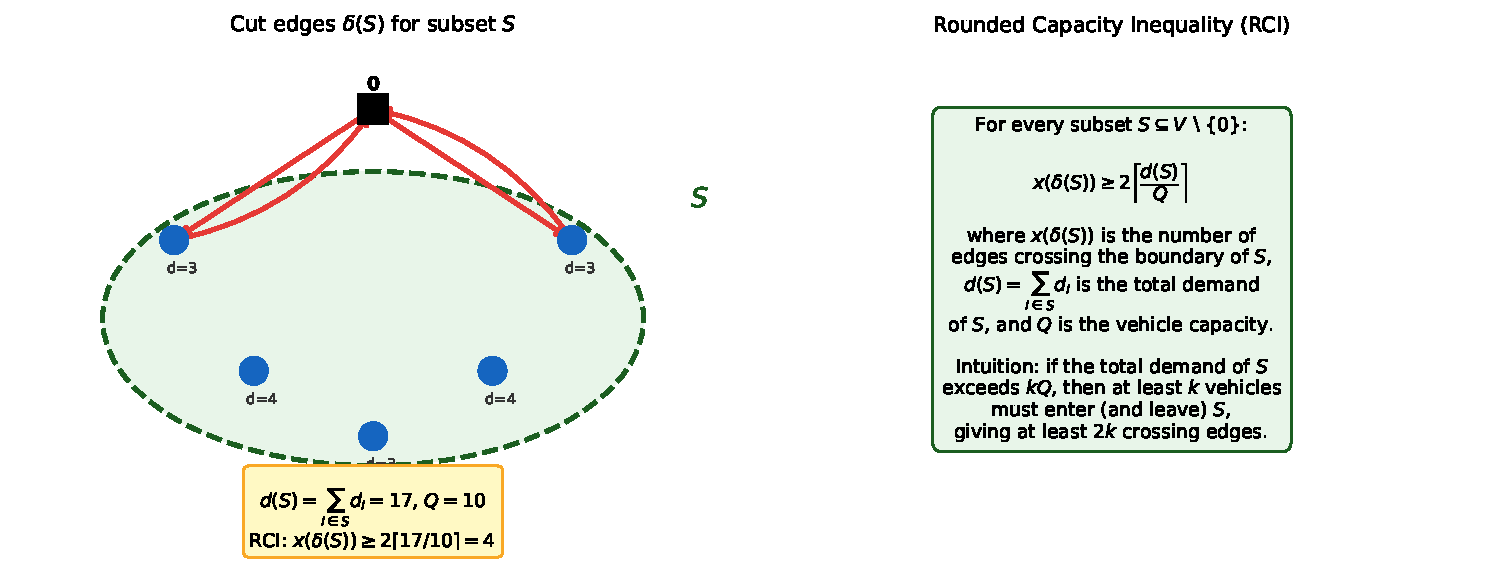
\includegraphics[width=\textwidth]{rounded_capacity}
    \end{column}
    \begin{column}{0.43\textwidth}
      \textbf{Left}: subset $S=\{1,2,3,4,5\}$ with total demand $d(S)=17$
      and $Q=10$. The RCI requires $x(\delta(S)) \geq 2\lceil 17/10\rceil=4$.
      The depot-to-$S$ boundary must be crossed by at least 4 arcs (two routes
      in, two routes out).
    \end{column}
  \end{columns}

  \framebreak

  \begin{block}{Generalised Capacity Inequalities (GCI)}
    The GCI proposed by Augerat et al.\ (1995) generalises the RCI by allowing
    a fractional multiplier. For $S \subseteq V'$:
    \[
      x(\delta(S)) \geq 2 \left\lceil \frac{\sum_{i\in S} d_i}{Q} \right\rceil.
    \]
    When customers have different demands, the GCI can be stronger than the
    RCI because the ceiling operation is applied to the \emph{sum} of demands
    rather than individual demands. In practice, the RCI and GCI coincide
    unless fractional demands are involved, but the GCI is the standard
    formulation used in the literature.
  \end{block}

  \bigskip
  The \emph{strengthened} version of the GCI incorporates a tighter right-hand
  side by exploiting the fact that each vehicle can carry at most $Q$ units:
  for any vertex $v \in S$, the GCI can be strengthened to:
  \[
    x(\delta(S)) + x(\delta(S\setminus\{v\})) \geq 4r(S) - 2r(S\setminus\{v\}).
  \]

  \framebreak

  \begin{block}{Framed Capacity Inequalities (FCI)}
    Introduced by Toth and Vigo (2002), the FCI extends the RCI by
    considering a \emph{frame} around subset $S$: a set $F$ of vertices
    ``surrounding'' $S$. Formally, for $S \subseteq V'$ and
    $F \supseteq S$ with $F \neq \emptyset$:
    \[
      x(\delta(S)) \geq 2r(S) + 2r(F\setminus S) - r(F).
    \]
    The FCI is at least as strong as the RCI when $r(F\setminus S) > 0$,
    because the right-hand side $2r(S) + 2r(F\setminus S) - r(F)$
    $\geq 2r(S)$ whenever routing $F\setminus S$ requires additional vehicles.
    These inequalities are generated by a separation procedure based on
    solving auxiliary LP sub-problems.
  \end{block}

  \framebreak

  \begin{block}{Hypotour Inequalities}
    Proposed by Gendreau, Laporte, and Seguin (1995), the hypotour
    inequality uses the concept of a ``hyper-tour''---a Hamiltonian cycle
    visiting some customers multiple times to respect capacity. For a subset
    $S \subseteq V'$, the hypotour inequality reads:
    \[
      x(E(S)) \leq |S| - r(S).
    \]
    Here $x(E(S))$ is the number of edges with both endpoints in $S$. The
    inequality says: if $r(S)$ vehicles service $S$, then at most $|S|-r(S)$
    arcs can be \emph{interior} to $S$ (the remaining arcs must connect to
    other vertices or the depot). When $r(S)=1$ this reduces to the standard
    sub-tour elimination constraint $x(E(S)) \leq |S|-1$.
  \end{block}

  \framebreak

  \begin{block}{Multistar Inequalities}
    Proposed by Augerat et al.\ (1995), the multistar inequality strengthens
    the RCI by incorporating individual customer degree constraints.
    For $S \subseteq V'$ with $|S| \geq 2$:
    \[
      x(\delta(S)) \geq 2r(S) + \max_{v \in S}\bigl(2r(S) - x(\delta(S\setminus\{v\}))\bigr).
    \]
    The term $2r(S) - x(\delta(S\setminus\{v\}))$ measures how much more
    the removal of the ``hardest-to-cover'' vertex $v$ from $S$ tightens
    the bound. This family was found to be very effective in practice by
    Lysgaard et al.\ (2004).
  \end{block}

  \framebreak

  \begin{block}{Comb Inequalities}
    Generalising the classic TSP comb inequalities (Chv\'atal, 1973) to the
    CVRP. A \emph{comb} consists of a \emph{handle} $H \subseteq V$ and an
    odd number $t \geq 3$ of \emph{teeth} $T_1,\ldots,T_t \subseteq V$
    satisfying:
    \begin{itemize}
      \item $H \cap T_k \neq \emptyset$ for all $k$ (each tooth intersects the handle),
      \item $T_k \setminus H \neq \emptyset$ for all $k$ (each tooth extends outside $H$),
      \item $T_k \cap T_\ell = \emptyset$ for $k \neq \ell$ (teeth are disjoint).
    \end{itemize}
    The comb inequality is:
    \[
      x(\delta(H)) + \sum_{k=1}^{t} x(\delta(T_k))
      \geq 3t + 1.
    \]
    This generalises to the CVRP context by the observation that routes must
    enter and leave both the handle and each tooth multiple times.
  \end{block}

  \framebreak

  \begin{columns}
    \begin{column}{0.52\textwidth}
      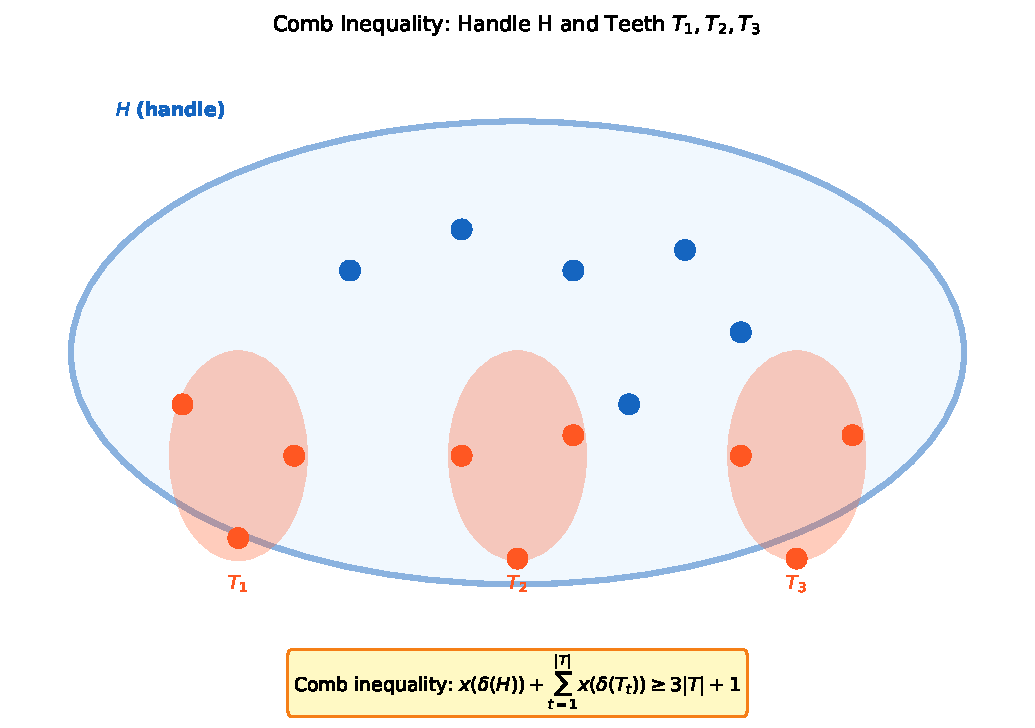
\includegraphics[width=\textwidth]{comb_inequality}
    \end{column}
    \begin{column}{0.46\textwidth}
      \textbf{Comb structure} with handle $H$ (blue ellipse) and three teeth
      $T_1, T_2, T_3$ (orange ellipses). Each tooth partially overlaps with
      the handle. The comb inequality requires:
      \[
        x(\delta(H)) + x(\delta(T_1)) + x(\delta(T_2)) + x(\delta(T_3))
        \geq 3 \times 3 + 1 = 10.
      \]
      Fractional LP solutions frequently violate this bound, and adding it
      typically raises the LP lower bound by 2--5\%.
    \end{column}
  \end{columns}

  \framebreak

  \begin{alertblock}{Key Insight: Which Cuts Are Most Effective?}
    Computational experiments by Lysgaard, Letchford, and Eglese (2004)
    on benchmark CVRP instances (E-instances of Christofides and Eilon, 1969)
    show that:
    \begin{enumerate}
      \item \textbf{RCI/GCI} are always applied first; they are cheap to
            separate (polynomial-time exact separation via minimum cut).
      \item \textbf{Framed capacity inequalities} provide the biggest
            improvement in LP bound per separation call.
      \item \textbf{Multistar and hypotour} inequalities are very effective
            but require more expensive separation.
      \item \textbf{Comb} and other TSP-type inequalities are used for the
            hardest instances.
    \end{enumerate}
    Using all four families, the B\&C of Lysgaard et al.\ (2004) solves
    E-instances up to $n=135$ customers routinely and set records for many
    benchmark instances.
  \end{alertblock}
\end{frame}

%% ============================================================
\section{Separation Procedures}
%% ============================================================

\begin{frame}[allowframebreaks]{2.4.2 Separation Procedures}
  A \emph{separation procedure} takes the current LP solution $x^*$ and
  either (a) finds a valid inequality violated by $x^*$ (i.e., a \emph{cut}),
  or (b) certifies that no such inequality exists in the chosen family.
  The efficiency and quality of separation procedures is crucial: if
  separation is too slow, the B\&C overhead outweighs the benefit of cuts.

  \bigskip
  \textbf{Separation for RCI/GCI.} Finding the most violated RCI requires
  solving a \emph{minimum $(s,t)$-cut} problem: choose $S$ to minimise
  $x(\delta(S)) - 2r(S)$. This is done as follows:
  \begin{enumerate}
    \item Build a capacitated graph where arc $(i,j)$ has capacity $x^*_{ij}$.
    \item For each customer $i$, run a minimum cut between $i$ and the depot 0.
          The minimum cut gives the subset $S$ minimising $x^*(\delta(S))$;
          check if $x^*(\delta(S)) < 2r(S)$.
    \item Use Gomory-Hu trees (Padberg and Rinaldi, 1990) to compute all
          pairwise minimum cuts efficiently in $O(n)$ max-flow calls.
  \end{enumerate}

  \framebreak

  \textbf{Separation for Framed Capacity Inequalities.}
  The separation procedure for FCI, described by Toth and Vigo (2002),
  solves a series of minimum-cut sub-problems with modified capacities to
  find the subset $S$ and frame $F$ yielding the most violated FCI. While
  more expensive than RCI separation, it is still polynomial.

  \bigskip
  \textbf{Separation for Comb Inequalities.}
  Exact separation of all comb inequalities is NP-hard in general.
  In practice, heuristic procedures are used:
  \begin{itemize}
    \item \textbf{Template-based search}: identify candidate handles from
          the fractional solution graph (highly fractional connected components).
    \item \textbf{Shrinking}: merge vertices with $x^*_{ij}$ close to 1,
          reducing the graph before searching for combs.
    \item \textbf{Sequential lifting}: start with a violated RCI as handle;
          find teeth that maximise violation.
  \end{itemize}
  These heuristics are not guaranteed to find all violated combs but work
  very well on benchmark instances.

  \framebreak

  \textbf{Separation for Multistar Inequalities.}
  Lysgaard et al.\ (2004) propose an exact polynomial separation for
  multistar inequalities based on the observation that the most violated
  multistar corresponds to maximising a quadratic function over a
  neighbourhood of the current LP solution. This can be solved efficiently
  using a sequence of minimum-cut computations.

  \bigskip
  \begin{block}{Summary of Separation Complexity}
    \begin{tabular}{lll}
      \toprule
      Inequality family & Separation complexity & Reference \\
      \midrule
      RCI / GCI         & Polynomial (min-cut)  & Padberg \& Rinaldi 1991 \\
      Framed capacity   & Polynomial (min-cut)  & Toth \& Vigo 2002 \\
      Hypotour          & Polynomial (LP)       & Gendreau et al.\ 1995 \\
      Multistar         & Polynomial            & Lysgaard et al.\ 2004 \\
      Comb              & NP-hard (heuristic)   & Padberg \& Rinaldi 1991 \\
      \bottomrule
    \end{tabular}
  \end{block}

  \framebreak

  \begin{alertblock}{Key Insight: The Cutting Plane Cycle}
    In B\&C, at each node one iterates the \emph{cutting plane cycle}:
    solve LP $\to$ separate $\to$ add cuts $\to$ re-solve LP $\to \ldots$
    until either (a) no violated inequality is found, (b) the LP solution
    becomes integer, or (c) a limit on the number of cuts per node is reached.
    The cycle typically terminates after 5--20 rounds at the root node,
    raising the LP bound by 10--30\% compared to the bare LP relaxation.
    At other nodes, reusing cuts from the parent accelerates convergence.
  \end{alertblock}
\end{frame}

%% ============================================================
\section{Comparison of B\&C Methods}
%% ============================================================

\begin{frame}[allowframebreaks]{2.4.3 Comparison of Branch-and-Cut Algorithms}
  Several B\&C algorithms have been proposed for the CVRP since the
  mid-1980s, progressively solving larger instances. We summarise the
  landmark algorithms and their key characteristics.

  \bigskip
  \begin{columns}
    \begin{column}{0.55\textwidth}
      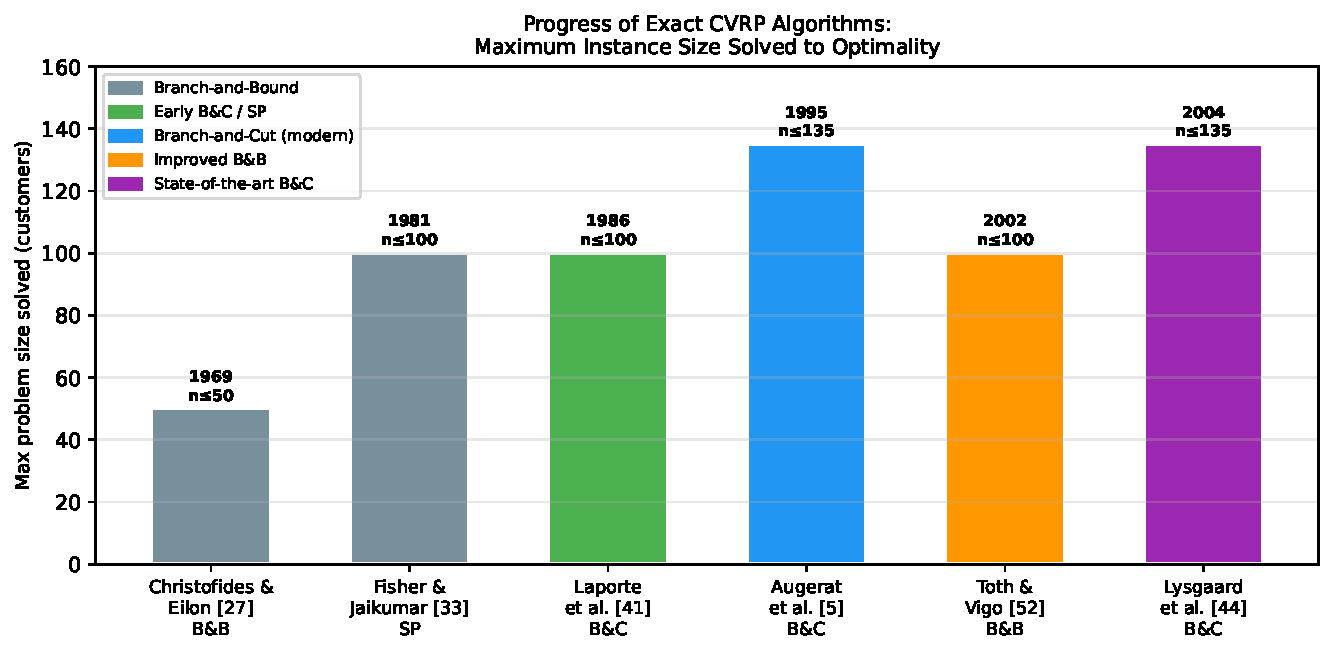
\includegraphics[width=\textwidth]{benchmark_comparison}
    \end{column}
    \begin{column}{0.43\textwidth}
      The figure shows the maximum CVRP instance size solved to proven
      optimality by each major algorithm, from 1969 to 2004. Progress
      has been roughly linear on a log scale: roughly doubling the
      instance size every decade, driven by better cutting planes and
      faster hardware.
    \end{column}
  \end{columns}

  \framebreak

  \begin{block}{Key Exact Algorithms: A Timeline}
    \begin{tabular}{lp{3.2cm}p{6cm}}
      \toprule
      Year & Authors & Key contribution \\
      \midrule
      1969 & Christofides \& Eilon & First B\&B with AP bound; $n \leq 50$ \\
      1981 & Fisher \& Jaikumar   & SP with generalised assignment; $n \leq 100$ \\
      1986 & Laporte et al.        & B\&C with RCI; $n \leq 100$ \\
      1989 & Agarwal et al.        & SP column generation; $n \leq 45$ \\
      1995 & Augerat et al.        & B\&C with GCI + multistar; $n \leq 135$ \\
      2002 & Toth \& Vigo          & Improved B\&B; $n \leq 100$ \\
      2004 & Lysgaard et al.       & CVRPSEP: full cut library; $n \leq 135$+ \\
      \bottomrule
    \end{tabular}
  \end{block}

  \framebreak

  \textbf{The CVRPSEP library.} Lysgaard, Letchford, and Eglese (2004)
  developed CVRPSEP, a publicly available library implementing separation
  routines for all major CVRP valid inequalities. Their B\&C algorithm uses:
  \begin{itemize}
    \item \textbf{LP relaxation} solved by CPLEX at every node.
    \item \textbf{Cutting plane cycle} with RCI, multistar, hypotour, and
          comb separation.
    \item \textbf{Branching} on the most fractional arc variable.
    \item \textbf{Best-first} node selection with occasional depth-first dives.
  \end{itemize}
  On the standard E-instances of Christofides and Eilon (sizes 22 to 101),
  they solved all instances to optimality in under 100 seconds on a 1.4 GHz
  machine. On larger CMT instances (Christofides, Mingozzi, Toth), they solved
  all instances up to $n=199$ within reasonable time limits, setting new
  records.

  \framebreak

  \textbf{The algorithm of Naddef and Rinaldi (2002).} Working independently,
  Naddef and Rinaldi developed a B\&C based on the symmetric TSP formulation
  with additional capacity cuts. They used a fractional relaxation combined
  with cutting planes derived from the polyhedral theory of the symmetric
  TSP. Their algorithm solved the 135-customer instance ``E101-k8'' to
  optimality, which had been open for many years.

  \bigskip
  \textbf{The algorithm of Baldacci, Christofides, and Mingozzi (2008).}
  A subsequent breakthrough was achieved by using an entirely different
  bounding approach: the \emph{state-space relaxation} combined with
  ng-route relaxations in a column-generation framework. This algorithm,
  not a pure B\&C, proved optimality for all standard benchmark instances
  up to $n=200$ customers.

  \framebreak

  \begin{exampleblock}{Example: Solving an E-instance}
    Consider instance E-n22-k4 (22 customers, 4 vehicles, from Christofides
    and Eilon, 1969). The LP relaxation at the root node gives a lower bound
    of, say, 373.4. The heuristic upper bound is 381. After the cutting-plane
    cycle at the root:
    \begin{enumerate}
      \item 8 RCI cuts raise LB to 376.2.
      \item 3 framed capacity cuts raise LB to 378.5.
      \item 1 comb cut raises LB to 380.1.
    \end{enumerate}
    Now LB=380.1 and UB=381, giving a gap of only 0.24\%. B\&C branches
    once, the child node LP gives 381.0, and the integer solution is confirmed
    as optimal. Total: 1 LP at root + 8 cuts + 1 branch = very fast.
  \end{exampleblock}
\end{frame}

%% ============================================================
\section{Conclusions and Future Directions}
%% ============================================================

\begin{frame}[allowframebreaks]{2.5 Conclusions and Future Research Directions}
  This chapter has reviewed the main exact algorithmic approaches for the
  CVRP, from the early B\&B methods of the late 1960s to the state-of-the-art
  B\&C algorithms of the 2000s. Several key conclusions emerge.

  \bigskip
  \textbf{Progress and current state.} The progress in exact CVRP algorithms
  has been substantial: from $n \leq 50$ in 1969 to $n \leq 199$ in 2008,
  a fourfold increase in problem size. This progress has been driven primarily
  by:
  \begin{enumerate}
    \item Better formulations (arc-variable, set partitioning).
    \item Tighter lower bounds (LP relaxations, column generation).
    \item Richer families of valid inequalities (RCI, comb, multistar).
    \item Faster computers (Moore's law).
  \end{enumerate}

  \framebreak

  \textbf{Remaining challenges.} Despite this progress, several open problems
  remain:
  \begin{itemize}
    \item \textbf{Larger instances}: instances with $n > 200$ customers remain
          very challenging, even for the best exact algorithms.
    \item \textbf{Stronger lower bounds}: the gap between the LP relaxation
          and the integer optimum is sometimes 5--15\% for large instances,
          suggesting many cutting planes are still missing from current libraries.
    \item \textbf{Asymmetric CVRP}: extensions to directed arcs and
          asymmetric cost matrices are harder; less progress has been made.
    \item \textbf{CVRP variants}: exact algorithms for CVRPTW, multi-depot
          CVRP, and other variants are less developed.
  \end{itemize}

  \framebreak

  \textbf{Future research directions.}
  The authors identify several promising directions:
  \begin{enumerate}
    \item \textbf{New valid inequalities}: deriving deeper cuts from the
          polyhedral structure of the CVRP, possibly combining capacity and
          routing constraints.
    \item \textbf{Improved pricing subproblems}: more efficient algorithms
          for the ESPPRC, the bottleneck in column-generation-based B\&C.
    \item \textbf{Parallel B\&C}: exploiting multi-core and cluster computing
          to explore multiple nodes simultaneously.
    \item \textbf{Hybrid methods}: combining exact B\&C with metaheuristics
          (matheuristics) to provide tight bounds for instances beyond the
          reach of pure exact methods.
    \item \textbf{Machine learning}: using ML to learn branching strategies,
          cut selection policies, and pricing heuristics, as has been done
          for general MIP solvers.
  \end{enumerate}

  \framebreak

  \begin{alertblock}{Overall Takeaway}
    The CVRP is one of the most intensively studied combinatorial optimisation
    problems, and the development of exact algorithms has produced a rich body
    of mathematical theory (polyhedral theory, column generation, cutting
    planes) with wide applicability beyond routing. The Branch-and-Cut
    paradigm, enriched with a comprehensive library of valid inequalities and
    efficient separation routines, remains the state of the art for proving
    CVRP optimality. Future advances will likely come from a combination of
    stronger mathematical structure, better algorithms for subproblems, and
    the integration of machine learning techniques.
  \end{alertblock}
\end{frame}

%% ============================================================
\section{Bibliography}
%% ============================================================

\begin{frame}[allowframebreaks]{Selected Bibliography}
  The following references are cited in Chapter 2. They are organised
  chronologically to illustrate the progression of the field.

  \begin{thebibliography}{99}
    \bibitem{CE69}
      P.~Christofides and S.~Eilon, ``An algorithm for the vehicle-dispatching
      problem,'' \textit{Operational Research Quarterly}, 20 (1969), pp.~309--318.

    \bibitem{FJ81}
      M.L.~Fisher and R.~Jaikumar, ``A generalised assignment heuristic for
      vehicle routing,'' \textit{Networks}, 11 (1981), pp.~109--124.

    \bibitem{CMT81}
      N.~Christofides, A.~Mingozzi, and P.~Toth, ``Exact algorithms for the
      vehicle routing problem, based on spanning tree and shortest path
      relaxations,'' \textit{Mathematical Programming}, 20 (1981), pp.~255--282.

    \bibitem{LMN86}
      G.~Laporte, H.~Mercure, and Y.~Nobert, ``An exact algorithm for the
      asymmetrical capacitated vehicle routing problem,'' \textit{Networks},
      16 (1986), pp.~33--46.

    \bibitem{AMS89}
      Y.~Agarwal, K.~Mathur, and H.M.~Salkin, ``A set-partitioning-based exact
      algorithm for the vehicle routing problem,'' \textit{Networks}, 19 (1989),
      pp.~731--749.

    \bibitem{Au95}
      P.~Augerat, J.M.~Belenguer, E.~Benavent, A.~Corber\'an, D.~Naddef,
      and G.~Rinaldi, ``Computational results with a branch-and-cut code for
      the capacitated vehicle routing problem,'' Research Report 949-M, 1995.

    \bibitem{GL95}
      M.~Gendreau, G.~Laporte, and R.~Seguin, ``A tabu search heuristic for
      the vehicle routing problem,'' \textit{Management Science}, 40 (1994),
      pp.~1276--1290.

    \bibitem{TV02}
      P.~Toth and D.~Vigo, ``Models, relaxations and exact approaches for the
      capacitated vehicle routing problem,'' \textit{Discrete Applied Mathematics},
      123 (2002), pp.~487--512.

    \bibitem{LLE04}
      J.~Lysgaard, A.N.~Letchford, and R.W.~Eglese, ``A new branch-and-cut
      algorithm for the capacitated vehicle routing problem,''
      \textit{Mathematical Programming}, 100 (2004), pp.~423--445.

    \bibitem{NR02}
      D.~Naddef and G.~Rinaldi, ``Branch-and-cut algorithms for the capacitated
      VRP,'' in \textit{The Vehicle Routing Problem}, P.~Toth and D.~Vigo, eds.,
      SIAM, 2002, pp.~53--84.

    \bibitem{BCM08}
      R.~Baldacci, N.~Christofides, and A.~Mingozzi, ``An exact algorithm for
      the vehicle routing problem based on the set partitioning formulation
      with additional cuts,'' \textit{Mathematical Programming}, 115 (2008),
      pp.~351--385.

    \bibitem{BMR11}
      R.~Baldacci, A.~Mingozzi, and R.~Roberti, ``New route relaxation and
      pricing strategies for the vehicle routing problem,''
      \textit{Operations Research}, 59 (2011), pp.~1269--1283.
  \end{thebibliography}
\end{frame}

%% ============================================================
%% Appendix: Python Implementation Sketches
%% ============================================================

\appendix

\begin{frame}[fragile]{Appendix A: CVRP Data Structures in Python}
  The following Python code defines the basic data structures for
  representing a CVRP instance and computing the objective value
  of a solution.

\begin{lstlisting}[language=Python, caption={CVRP instance and solution evaluation}]
import numpy as np
from dataclasses import dataclass, field
from typing import List, Dict

@dataclass
class CVRPInstance:
    """
    A CVRP instance.
    n        : number of customers (vertices 1..n; 0 = depot)
    coords   : (n+1) x 2 array, coords[0] = depot
    demands  : length-(n+1) array; demands[0] = 0
    capacity : vehicle capacity Q
    """
    n: int
    coords: np.ndarray  # shape (n+1, 2)
    demands: np.ndarray # shape (n+1,)
    capacity: float

    def cost_matrix(self) -> np.ndarray:
        """Euclidean distance matrix (n+1) x (n+1)."""
        diff = self.coords[:, None, :] - self.coords[None, :, :]
        return np.sqrt((diff**2).sum(axis=2))

def route_cost(instance: CVRPInstance, route: List[int]) -> float:
    """
    Cost of a single route (list of customers, depot implicit).
    E.g. route=[1,3,2] means 0->1->3->2->0.
    """
    C = instance.cost_matrix()
    path = [0] + route + [0]
    return sum(C[path[i], path[i+1]] for i in range(len(path)-1))

def solution_cost(instance: CVRPInstance,
                  routes: List[List[int]]) -> float:
    """Total cost of a CVRP solution (list of routes)."""
    return sum(route_cost(instance, r) for r in routes)

def is_feasible(instance: CVRPInstance,
                routes: List[List[int]]) -> bool:
    """Check: every customer visited once, capacity respected."""
    visited = []
    for r in routes:
        if sum(instance.demands[i] for i in r) > instance.capacity:
            return False
        visited.extend(r)
    return sorted(visited) == list(range(1, instance.n+1))
\end{lstlisting}
\end{frame}

\begin{frame}[fragile]{Appendix B: Greedy Nearest-Neighbour Heuristic (Upper Bound)}
  Before running exact B\&C, a quick heuristic is needed to provide an
  initial upper bound. The nearest-neighbour heuristic greedily constructs
  routes by always visiting the nearest unvisited customer.

\begin{lstlisting}[language=Python, caption={Nearest-neighbour heuristic for CVRP}]
def nearest_neighbour_cvrp(inst: CVRPInstance
                           ) -> List[List[int]]:
    """
    Greedy nearest-neighbour CVRP heuristic.
    Returns a list of routes (each route = list of customer indices).
    """
    C = inst.cost_matrix()
    unvisited = set(range(1, inst.n + 1))
    routes = []

    while unvisited:
        route = []
        load = 0.0
        current = 0  # start at depot

        while unvisited:
            # Find nearest feasible unvisited customer
            best = None
            best_dist = float('inf')
            for j in unvisited:
                if (load + inst.demands[j] <= inst.capacity
                        and C[current, j] < best_dist):
                    best = j
                    best_dist = C[current, j]
            if best is None:
                break  # no feasible customer; close route
            route.append(best)
            load += inst.demands[best]
            unvisited.discard(best)
            current = best

        if route:
            routes.append(route)

    return routes

# --- Example usage ---
np.random.seed(42)
n = 8
coords = np.vstack([[0, 0],           # depot
                    np.random.rand(n, 2) * 10])
demands = np.array([0] + [2, 3, 1, 4, 2, 3, 1, 2])
inst = CVRPInstance(n=n, coords=coords,
                    demands=demands, capacity=8)
routes = nearest_neighbour_cvrp(inst)
print(f"Routes: {routes}")
print(f"Total cost: {solution_cost(inst, routes):.2f}")
print(f"Feasible: {is_feasible(inst, routes)}")
\end{lstlisting}
\end{frame}

\begin{frame}[fragile]{Appendix C: Rounded Capacity Inequality Separation}
  The following code implements a simple exact separation procedure for
  the Rounded Capacity Inequality (RCI) using a minimum-cut approach.

\begin{lstlisting}[language=Python, caption={RCI separation using minimum cut (simplified)}]
import networkx as nx
import math
from itertools import combinations

def separate_rci(inst: CVRPInstance,
                 x_frac: Dict) -> List[tuple]:
    """
    Separate Rounded Capacity Inequalities.
    x_frac: dict {(i,j): x*_{ij}} fractional LP solution.
    Returns list of violated RCIs as (S, lhs, rhs) tuples.
    """
    violations = []
    n = inst.n

    # Build a graph with LP solution values as capacities
    G = nx.Graph()
    for (i, j), val in x_frac.items():
        if val > 1e-6:
            G.add_edge(i, j, capacity=val)

    # For each customer k, find min cut between k and depot 0
    for k in range(1, n + 1):
        if k not in G or 0 not in G:
            continue
        try:
            cut_val, (S_side, T_side) = nx.minimum_cut(G, k, 0)
        except nx.NetworkXError:
            continue

        # S = customer side of cut (excluding depot)
        S = {v for v in S_side if v != 0}
        if not S:
            continue

        d_S = sum(inst.demands[i] for i in S)
        rhs = 2 * math.ceil(d_S / inst.capacity)

        # Count fractional arcs crossing delta(S)
        lhs = sum(val for (i, j), val in x_frac.items()
                  if (i in S) != (j in S))  # XOR = crosses boundary

        if lhs < rhs - 1e-4:
            violations.append((S, lhs, rhs))

    return violations

# Example: check a fractional solution
x_star = {(0,1): 0.7, (1,2): 0.5, (2,0): 0.6,
           (0,3): 0.8, (3,0): 0.5}
# (demo only -- inst from Appendix A)
\end{lstlisting}
\end{frame}

\begin{frame}[fragile]{Appendix D: Branch-and-Bound Skeleton}
  The following code provides a skeleton implementation of a simple
  Branch-and-Bound algorithm for CVRP, illustrating the key components
  discussed in the chapter. This is a conceptual implementation;
  a production solver would use an LP solver (e.g., CPLEX or Gurobi)
  and a much richer set of cutting planes.

\begin{lstlisting}[language=Python, caption={Branch-and-Bound skeleton for CVRP}]
from heapq import heappush, heappop

def branch_and_bound_cvrp(inst: CVRPInstance,
                          compute_lb,   # callable: node -> lb
                          get_heuristic # callable: inst -> routes
                          ):
    """
    Minimalist B&B skeleton for CVRP.
    compute_lb(node)   -> float: lower bound for node subproblem
    get_heuristic(inst)-> routes: initial UB
    """
    # Initialise
    init_routes = get_heuristic(inst)
    UB = solution_cost(inst, init_routes)
    best_solution = init_routes

    # Priority queue: (lb, node_id, node_data)
    node_id = 0
    root = {'fixed_1': [], 'fixed_0': []}  # fixed arcs
    open_list = []
    heappush(open_list, (0.0, node_id, root))

    while open_list:
        lb, nid, node = heappop(open_list)

        # Pruning by bound
        if lb >= UB - 1e-6:
            continue

        # Compute tighter LB (LP or AP relaxation)
        tight_lb = compute_lb(node)
        if tight_lb >= UB - 1e-6:
            continue

        # Check if LP solution is integer
        lp_sol = solve_lp(inst, node)  # placeholder
        if lp_sol is None:             # infeasible
            continue
        if is_integer(lp_sol):
            cost = solution_cost(inst, lp_sol)
            if cost < UB:
                UB = cost
                best_solution = lp_sol
            continue

        # Branch on most fractional arc
        frac_arc = most_fractional(lp_sol)
        for fix_val in [1, 0]:
            child = dict(node)
            if fix_val == 1:
                child['fixed_1'] = node['fixed_1']+[frac_arc]
            else:
                child['fixed_0'] = node['fixed_0']+[frac_arc]
            node_id += 1
            heappush(open_list, (tight_lb, node_id, child))

    return best_solution, UB
\end{lstlisting}
\end{frame}

\begin{frame}[allowframebreaks]{Appendix E: Valid Inequalities --- Summary Table}
  This table summarises all the valid inequality families discussed in
  the chapter, together with their key properties.

  \begin{center}
  \small
  \begin{tabular}{p{2.8cm}p{5.5cm}p{2.8cm}l}
    \toprule
    \textbf{Name} & \textbf{Form} & \textbf{Parameters} & \textbf{Separation} \\
    \midrule
    Rounded Capacity (RCI)
    & $x(\delta(S)) \geq 2\lceil d(S)/Q \rceil$
    & $S \subseteq V'$
    & Poly (min-cut) \\[6pt]
    Generalised Cap.\ (GCI)
    & $x(\delta(S)) \geq 2\lceil d(S)/Q \rceil$
    & $S \subseteq V'$
    & Poly (min-cut) \\[6pt]
    Framed Capacity (FCI)
    & $x(\delta(S)) \geq 2r(S)+2r(F\setminus S)-r(F)$
    & $S \subseteq F \subseteq V'$
    & Poly \\[6pt]
    Hypotour
    & $x(E(S)) \leq |S| - r(S)$
    & $S \subseteq V'$
    & Poly (LP) \\[6pt]
    Multistar
    & $x(\delta(S)) \geq 2r(S) + \max_v[\ldots]$
    & $S \subseteq V'$
    & Poly \\[6pt]
    Comb
    & $x(\delta(H))+\sum_k x(\delta(T_k)) \geq 3t+1$
    & Handle $H$, Teeth $T_k$
    & NP-hard (heuristic) \\
    \bottomrule
  \end{tabular}
  \end{center}

  \bigskip
  \textbf{How to read the table.}
  For each inequality family, the ``Form'' column gives the mathematical
  statement of the inequality, where $S$ (and $F$, $H$, $T_k$) are the
  subsets of customers that parametrise the family. The ``Separation''
  column indicates the computational complexity of finding the most violated
  inequality in the family given a fractional LP solution.
  ``Poly'' means a polynomial-time exact algorithm exists; ``NP-hard
  (heuristic)'' means exact separation is NP-hard, and heuristic procedures
  are used in practice.
\end{frame}

\end{document}
